The storm surge is generally defined as the difference between the observed mean sea level and the astronomical tide. To be more precise, one should specify the duration over which this average is performed. It is customary to take a long enough average so that the crest-to-trough variations due to wind waves (on a time scale under 30 s) are filtered out. In general, the longer infragravity with periods 20 to 300~s are also filtered. It is thus customary to write the instantaneous sea level at the coast as a sum of the tide, surge, and run-up, with the run-up containing all the oscillatory motions shorter than about 300~s. 

However, even if the water level oscillations caused by waves are filtered out, the storm surge does contain some direct effect of the waves: this is called the "wave set up". This wave set-up can be large part of the storm surge. For example, it was estimated to be about 1~m out of the 8~m of storm surge that flooded New Orleans during the passage of Hurricane Katrina in 2005  \citep{Resio&Westerink2008}. The proportion of set-up in the storm surge increases. On the French Atlantic coast, the highest storm surge recorded is around 4~m on the steep cliffs of Bannec Island near Molne \citep{Ardhuin&Magne2010,Sheremet&al.2014}. In that case the wave set-up exceeds 80\% of the storm surge. In the context of rising global sea level exacerbated by land subsidence in many coastal cities, understanding and managing the wave-induced extra meters of sea level will thus become more and more important. This, together with wave-induced currents that are the main source of nearshore sediment transport, are the main motivations for the present chapter. 

\section{Mean flow equations}
We have established in chapter \ref{ch_momentum} that waves introduce and extra flux of momentum, the radiation stress $S^{\mathrm{rad}}$ (which is a 2 by 2 tensor) and a mass flux, the Stokes transport ${\mathbf M^w}$ (\ref{Phillips_mass}) which is a horizontal vector. We have given in chapter \ref{ch_courant} the form of the wave-averaged momentum and mass conservation equations. We are now going to look at the consequences of these wave-induced fluxes in the surf zone. 

We recall  that the mean water depth is 
$D=\overline{\zeta}+h$ and the total mass flux caused by a mean current and the waves is  ${\mathbf M}=\rho
{\mathbf \hu} D +{\mathbf M}$. We also define the mean mass flux velocity to be  ${\mathbf U}={\mathbf
M}/\left(\rho D\right) = {\mathbf \hu}+{\mathbf M^w}/\left(\rho
D\right)$. 

Given the small spatial scales of the surf zone we can neglect the Coriolis force. Considering a stationary solution, the momentum equations  (\ref{Phillips_mom}) becomes 
\begin{equation}
\fbox{$\displaystyle \frac{\partial }{\partial x}\left(U_x M_x+S^{\mathrm{rad}}_{xx}\right)
    +\frac{\partial }{\partial y}\left(U_x M_y+S^{\mathrm{rad}}_{yx}\right)
     =  -\rho g D  \frac{\partial \overline{\zeta}}{\partial x}
        + \tau_{x,{\mathrm s}}  + \tau_{x,{\mathrm b}}$} \label{xmomentum}
\end{equation}
\begin{equation}
\fbox{$\displaystyle \frac{\partial }{\partial x}\left(U_y M_x+S^{\mathrm{rad}}_{xy}\right)
    +\frac{\partial }{\partial y}\left(U_y M_y+S^{\mathrm{rad}}_{yy}\right)
     =  -\rho g D  \frac{\partial \overline{\zeta}}{\partial y}
        + \tau_{y,{\mathrm s}}  + \tau_{y,{\mathrm b}}, $} \label{ymomentum}
\end{equation}
where $\left(\tau_{x,{\mathrm s}},\tau_{y,{\mathrm s}}\right)$ and
$\left(\tau_{y,{\mathrm b}},\tau_{y,{\mathrm b}}\right)$ are the surface and bottom stresses respectively.

\section{Mean sea level: set-down and set-up}
We now take the coast to be straight and aligned in the $y$ direction. Assuming that everything is uniform alongshore, all derivatives with respect to $y$ vanish. The mass conservation given by eq. (\ref{Phillips_mass})  thus becomes, 
\begin{equation}
  \frac{\partial M_x}{\partial x} = 0.
\end{equation}
In other words  $M_x$ is a constant, and since we expect no flow through the coast 
this constant is zero,  $M_x=0$.
We note that it means that the transport due to the mean current must be opposite to the 
Stokes transport. Since the Stokes drift is directed shoreward and concentrated near the surface this explains that the mean current is directed offshore: this current is also called the "undertow".

Momentum conservation in the cross-shore $x$ direction reads 
\begin{equation}
    \frac{\partial }{\partial x}S^{\mathrm{rad}}_{xx}
     =  -\rho g D \partial \frac{\overline{\zeta}}{\partial x}
        + \tau_{a,x}  + \tau_{b,x}
\end{equation}
For waves with crests parallel to the shore  $\theta =0$. If we first neglect the surface and bottom stress, $\tau_{a,x}=\tau_{b,x}=0$, we get a sloping sea level 
\begin{equation}
    \frac{\partial \overline{\zeta}}{\partial x}=
        -\frac{1}{\rho g D}\frac{\partial }{\partial x}
        \left[\frac{C_g E}{C}\left(2
        - \frac{\sinh 2kD}{\sinh 2kD +2kD}\right)\right].
\end{equation}
Even without computing the solution, we note that for waves which do not break the energy flux  $C_gE$ is constant, and given that the phase speed $C$ becomes smaller in shallower water, the flux  $S^{\mathrm{rad}}_{xx}$ increases in shallower water, which gives a negative ${\partial \overline{\zeta}}/{\partial x}$, meaning that the sea level decreases towards the shore: this is the "set-down". 
 For a first approximation one could assume $\overline{\zeta} << h$ and then replace $D$ with $h$, to obtain 
\begin{equation}
    \overline{\zeta}=-\frac{a^2k}{2\sinh\left(2kD\right)} \label{setdown}
\end{equation}
where $a$ is the local wave amplitude. To obtain this relation you can consider that 
the wave frequency is constant and take the derivative of $\sigma^2=gk\tanh kD$ to obtain a relationship between  ${\partial k}/{\partial x}$ and ${\partial
D}/{\partial x}$. Besides, using Snel's law one finds that this relation also holds for any wave direction offshore. 

At the location where waves start to break, with depth  $h_d$, we can assume that waves are in shallow water, i.e. $k D<<1$, giving a wave height $H_b=2a=\gamma h_d$ and thus a lowest elevation of the mean sea level
\begin{equation}
    \overline{\zeta}=-\frac{\gamma}{16}H_b.
\end{equation}
Using values in Fig. \ref{fig:surfer} for a 2~m  12~s swell with an incidence angle of 20$^\circ$ the breaking wave height is  $2.3$~m and taking  $\gamma=0.4$  we get a set-down of 6~cm.

Now, when waves break the flux generally decreases and the sea level goes up: this is the "set-up". In the surf zone, the wave height is controled by the local water depth, given roughly by $2a=H_b=\gamma D$ so that the energy density  is 
\begin{equation}
    E=\rho g \gamma^2 D^2/8.
\end{equation}
Assuming shallow water  $kD <<
1$ gives $S^{\mathrm{rad}}_{xx} =  1.5 E$ and 
\begin{equation}
    S^{\mathrm{rad}}_{xx}=\frac{3}{16}\rho g \gamma^2 \left(h+\overline{\zeta}\right)^2.
\end{equation}
Now replacing that in the momentum equation
\begin{equation}
    \frac{3}{16} \gamma^2 2\left(h+\overline{\zeta}\right)
    \frac{\partial}{\partial x} \left(h+\overline{\zeta}\right)
    =- \left(h+\overline{\zeta}\right)\frac{\partial \overline{\zeta}}{\partial x}
\end{equation}
we get the sea level slope
\begin{equation}
    \frac{\partial \overline{\zeta}}{\partial x}
    =- B \frac{\partial h}{\partial x}
\end{equation}
where
\begin{equation}
    B=\left[1+\frac{1}{3 \gamma^2/8}\right]^{-1}
\end{equation}
which integrates to 
\begin{equation}
    \overline{\zeta}
    =-B h + A_0.
\end{equation}
where $A_0$ is given by matching the set-down value at the depth $h_d$, 
\begin{equation}
    \overline{\zeta}
    =B \left(h_d-h\right) + \overline{\zeta}_d.
\end{equation}
The depth difference $\left(h_d-h\right)$ is positive in the surf zone and the wave set-up increases towards the shore. Using the same numerical values, 
(swell of offshore wave height 2~m), at the coast where $h=0$, we get  $\overline{\zeta}=26$~cm.

\subsection{Wave set-up in practice}
Measurements of mean sea level in the surf zone haev generaly confirmed the cross-shore momentum balance between the convergence of the radiation stresses and the slope in the mean sea level. However, in reality, bottom friction can be an important term for shallow water, in particular $D < 1~m$ in the examples shown in Fig. \ref{Apotsos_setup}. 
%%%%%%%%%%%%% figure
\begin{figure}
\centerline{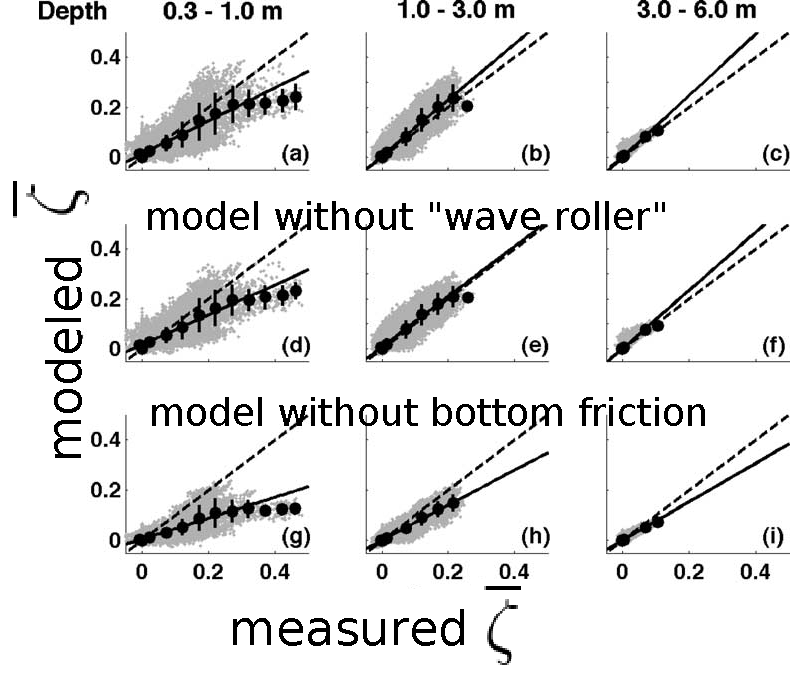
\includegraphics[width=0.7\textwidth]{FIGURES/Apotsos_setup.pdf}}
%\vspace{3.64in}
  \caption{Wave set up on the beach: measurements and model}
    {Data were collected from September to November at locations 10 to 300~m from the shoreline at Duck, North Carolina. The data was sliced into 8.5 minute-long records, and the figure shows the observed mean sea level compared to the prediction using a model that integrates gradients of radiation stresses, with radiation stresses estimated from local wave measurements. One flavor of the model includes a parameterization for a "wave roller" which is represents the wave roller as an intermediate buffer of momentum between the waves and the mean flow. Bottom friction is parameterized here with an eddy viscosity that is a function of he wave height, giving bottom drag coefficient valies close to those of eq. (\ref{taub_LH70}) 
avec un coefficient $0.018 <C_f< 0.028$
that is typically higher than values used for the longshore current, but which could be justified by the orientation of surfzone "megaripples" \citep{Gallagher&al.1998}. Picture from  \cite{Apotsos&al.2007}, copyright American Geophysical Union.}
\label{Apotsos_setup}
\end{figure}
%%%%%%%%%%%%% end of figure

Because the set-up (mean level) and run-up (which includes wave-by-wave oscillations) are a function of the details of the beach profile, which is often not known well enough, many alternative empirical methods have been proposed using a simplification of the beach shape and offshore wave parameters. The values of set-up and run-up are particularly important for understanding how far the sea can reach inland, and designing shoreline protection structures.  \cite{Hunt1959} considered a height parameter that combines the offshore wave period and offshore wave height, 
\begin{equation}
H_H=T_{m0,-1} \sqrt{g H_s},
\end{equation}
Many observations show that extreme water levels generally scale with this height $H_H$.  For a given depth profile, Fig. \ref{bannec_runup}  shows how $H_H$ gives a useful scale of extreme water levels measured at Bannec island (to be precise, the measurement is not a water level but a pressure converted to height above the sensor assuming hydrostatic equilibrium). 
%%%%%%%%%%%%% figure
\begin{figure}
\centerline{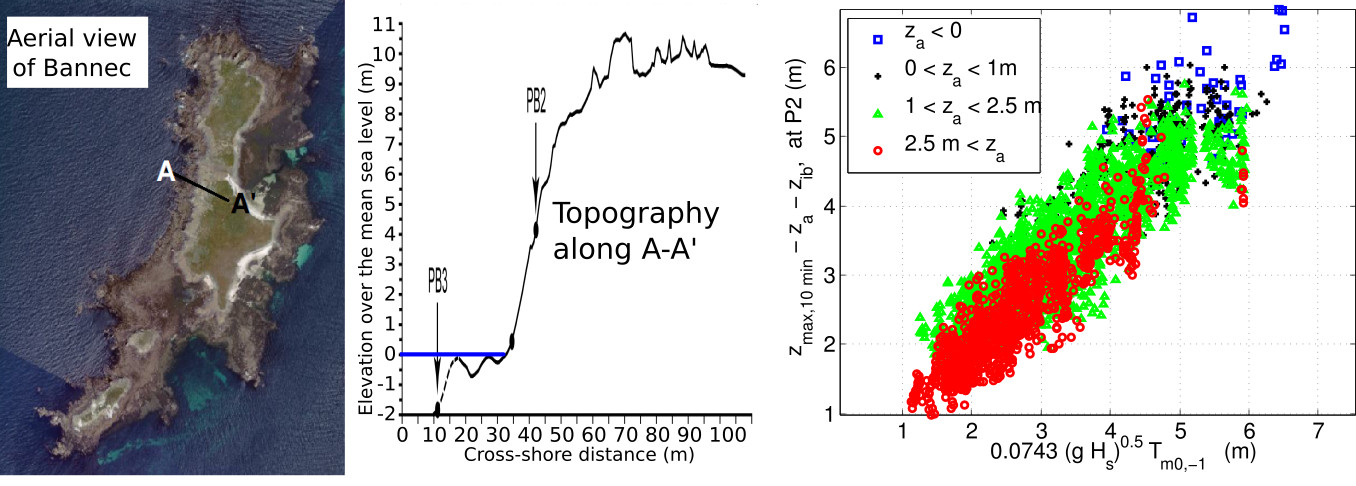
\includegraphics[width=\textwidth]{FIGURES/bannec_runup.jpg}}
%\vspace{3.64in}
  \caption{Left: map of Bannec island, Center: topography profile along the A-A' transect, Right: Maximum surface elevation for every 10-minute record from October 2008 to March 2009, as a function of the offshore wave height and period estimated from the wave model of \cite{Ardhuin&Magne2010}. Blue squares correspond to an astronomical tide below the mean sea level, and red squares are for tide levels above 2.5~m.}
\label{bannec_runup}
\end{figure}
%%%%%%%%%%%%% end of figure
This height parameter is also related to the Irribaren number introduced in chapter \ref{ch_surf}, indeed the set-up and run-up are also a function of the foreshore slope $\beta_f$ (the slope of the part of the beach that goes from dry to wet with the passage of the waves), so that the run-up can be written as proportional to the offshore wave height times the Irribaren number $\xi_0$. 

For example, \cite{Stockdon&al.2006} found an empirical relation of the form 
\begin{equation}
    \overline{\zeta} \simeq  0.14 \beta_f H_H
\end{equation}
This formula is semi-quantitative: it only explains half of the variance in the data collected by these authors, and up to 70\% of the variance for the most dissipative cases. In fact, for $\xi_0 < 0.3$, the slope appears secondary and this expression fits these cases better, 
\begin{equation}
    \overline{\zeta} \simeq  0.0064  H_H.
\end{equation}

Similar expression have been derived for the run-up \citep{Holman1986}, and recent analysis of pebble beaches \citep{Poate&al.2016} and cliffs \citep{Dodet&al.2018} show that they probably need to be adjusted for these environments. 
Further studies have also investigated how much water goes over a dune or coastal structure, which is really the quantity of interest for flooding where the coast is not erodible  \citep{EuroTop2007}. 


\section{The longshore current}
Now looking that the momentum balance in the along-shore $y$ direction, we get 
\begin{equation}
    \frac{\partial S^{\mathrm{rad}}_{xy}}{\partial x}
    = \tau_{y,{\mathrm s}}  + \tau_{y,{\mathrm b}} \label{ymomentum2}
\end{equation}
and for monochromatic waves with incidence angle $ \theta$ the radiation stress is 
\begin{equation}
    S^{\mathrm{rad}}_{xy}=E \frac{C_g}{C} \sin \theta \cos \theta .
\end{equation}
Since $\sin \theta/C$ is a constant according to Snel's law, the force exerted by waves along the $y$ axis is zero where $E C_g/\cos \theta$ is constant, which is outside the surf zone. However, inside the surf zone, the energy flux $E C_g/\cos \theta$  is reduced 
in the case $\sin \theta>0$ or augmented if 
$\sin \theta<0$. As a result, the divergence of $S_{xy}^{\mathrm{rad}}$ gives a force that pushes the water along the shore. If we neglect the wind stress, the bottom stress   $\tau_{y,{\mathrm b}}$ is the only force that can balance the wave-induced force. Since the bottom stress is in the opposite direction to the mean current, then there should be a current $V$ flowing towards $y>0$ in the case $\sin \theta>0$.

For a quantitative estimate, we may assume an instantatenous quadratic drag law, 
\begin{equation}
    {\mathbf T}\left(t\right)=-C_f
    \left|\left({\mathbf U}+{\mathbf u}\right)\right|
    \left({\mathbf U}+{\mathbf u}\right)
\end{equation}
\cite{Longuet-Higgins1970} showed that for
$\left|V\right|<< \overline{\left|u\right|}$  and small values of 
$\theta$, the bottom stress becomes
\begin{equation}
    \tau_{y,{\mathrm b}}=- \overline{\rho C_f \left|u\right|\left(V+v\right)}\label{taub_LH70}
\end{equation}
where $V$ is the mean current in the  $y$ direction and  $\left(u,v\right)$ is the orbital velocity at the sea floor. Using linear wave theory that gives 
\begin{eqnarray}
    u& =& \frac{gD}{2C}\cos\left(kx-\omega t\right)\\
      \overline{\left|u\right|} & =& \frac{gD}{\pi C}\\
    \tau_{y,{\mathrm f}}&=&-\rho C_f \frac{gD}{\pi C} V
\end{eqnarray}
and the longshore current velocity is given by \citep{Thornton&Guza1986}, 
\begin{equation}
    V=- \frac{\pi C}{\rho C_f  g D}
    \frac{ \partial \left(E C_g \cos \theta\right)}{\partial x}
    \frac{\sin \theta_0}{C_0}.\label{TG86}
\end{equation}

One example of estimated surf zone current for a beach profile that includes a bar is shown in Fig. \ref{fig:surfer_cur}. The large magnitude of the current, of the order of 1~m/s is realistic. This current has also been called the "river of sand" as it is responsible for transporting sand along beaches in the direction of the dominant waves. 
%%%%%%%%%%%%% figure
\begin{figure}[htb]
\centerline{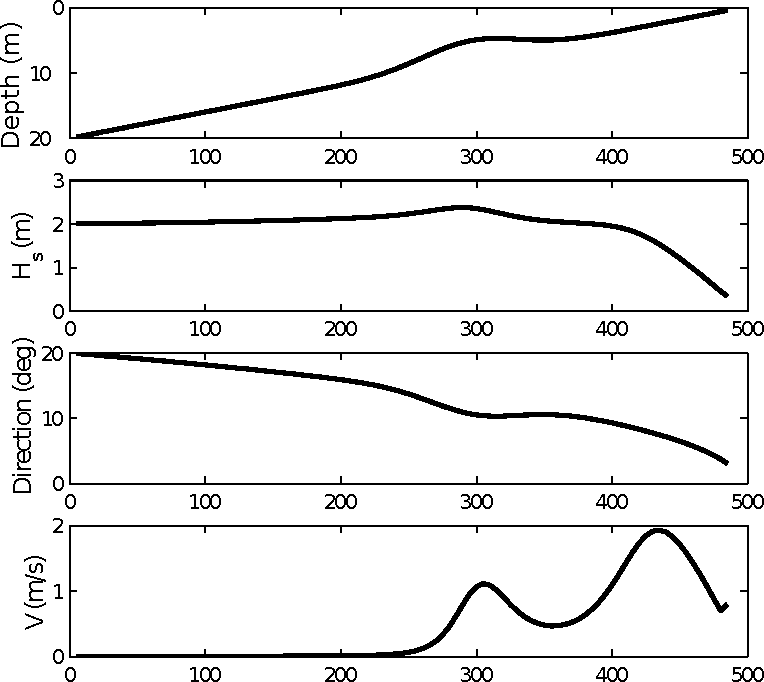
\includegraphics[width=0.5\textwidth]{FIGURES/surfer_cur.pdf}}
%\vspace{3.64in}
  \caption{Wave breaking and longshore current}
    {Results of the model by \cite{Thornton&Guza1986}  for the same case shown in Fig. \ref{fig:surfer}, namely a wave period $T=12$~s and 20$^\circ$ incidence angle 
    in 20~m depth. Waves propagate over a schematic beach with a mean slope $\beta=0.04$ 
    and a bar at $x=300$~m.}
\label{fig:surfer_cur}
\end{figure}
%%%%%%%%%%%%% end of figure
Sandy beaches are only in equilibrium when they are facing the waves, which qualitatively explains the usual concave shape of beaches (when seen from above) that naturally tends to realign itself to face the waves: this also explains the formation of tombolos behind detached breakwaters, and many other features. 

In practice, however, the spatial variation of the current on barred beaches does not generally have the two maxima in the longshore current (for example at 300~m and 430~m in Fig. \ref{fig:surfer_cur}) but rather one single broad maximum \citep{Reniers&Battjes1997}. Many reasons have been used to explain this: horizontal mixing by horizontal vortices \citep{Church&Thornton1993,Brocchini&al.2004}, the "buffering effect" of the "wave roller" \citep{Lippmann&al.1996}, or the mixing effect of vertical shear \citep{Putrevu&Svendsen1999}.  Also, the current is not a steady flow but instead is highly variable, due to the variability of the forcing itself and also related to instabilities of the current \citep{Oltman-Shay&al.1989}.


%L'équation (\ref{TG86}) est le modèle de Thornton et Guza (1986\nocite{Thornton&Guza1986}), qui utilise la dissipation d'énergie des vagues ${ \partial E C_g \cos \theta}/{\partial x}$ prévue par le modèle de transformation des vagues de Thornton et Guza (1983), décrit au paragraphe \ref{TG1983}. En revenant à nos vagues $H=2$~m, $T=12$~s et  $\theta_0=20^{\circ}$, on trouve une valeur maximale du courant de 2 m~s$^{-1}$ (voir figure \ref{surfer}). Ce modèle comporte assez de paramètres `libres', en particulier $C_f$ (on peut `bidouiller') pour permettre de reproduire les observations. Les premières vérifications furent faites  lors de l'expérience NSTS (Nearshore Sediment Transport Study) en 1980, sur les plages de Torrey Pines (au Nord de San Diego) et Leadbetter (Santa  Barbara). L'hypothèse $\left|V\right|<< \overline{\left|u\right|}$ faite par Longuet-Higgins (1970) pour la forme paramétrée de la tension est assez dérisoire car pour une couche limite oscillante (chapitre 3), la tension n'est plus tout à fait quadratique, cela n'a pas empêché Thornton et Guza (1986) d'étudier en détail l'effet de la non-linéarité de $\tau_y$ en fonction de $V$ quand $V \sim \overline{\left|u\right|}$. On peut améliorer le modèle en ajoutant une diffusion horizontale de quantité de mouvement qui réduira un peu les gradients de $V$. Beaucoup de travail a aussi été fait récemment sur le mécanisme exact du transfert de quantité de mouvement entre les vagues et le courant. Il a en particulier été mis en évidence que le "rouleau" (le paquet d'écume transporté par une vague qui déferle) pouvait jouer le rôle d'un "tampon à quantité de mouvement" et retarder le transfert entre les vagues et le courant.

\section{Cross-shore flows}
Besides the along-shore transport of material, and in particular sediments, surf zones are also active regions of cross-shore exchanges. Part of this exchange is associated to the vertical profile of the cross-shore current, with an onshore flow in the wave bottom boundary layer, associated to streaming \citep{Longuet-Higgins1953}, an offshore flow above the boundary layer and onshore transport related to the Stokes drift near the surface.  

The other part of the cross-shore flow is related to non-stationarity and non-uniformities of the surf zone currents. Figure \ref{fig:surf_pink} shows two examples of the transport of water marked by the fluorescent tracer rhodamine which appears in pink. The tracer was released at a single point in the surf zone or near the mouth of a river during the ebb flow. 
The tracer is clearly transported along the coast by the longshore current and also mixed across the surf zone. This has clear implications for the sediment transport and the transport of contaminant around beaches which is important for water quality and human health \citep{Delpey&al.2014}.


 Entrainment of material further offshore is of particular interest for fisheries (larvae recruitment), the global carbon cycle, or plastic contamination of the ocean. Waves are again important right at the surface or in the shallower parts of the continental shelf \citep{Lentz&al.2008,Onink&al.2019}.

%%%%%%%%%%%%% figure
\begin{figure}[htb]
\centerline{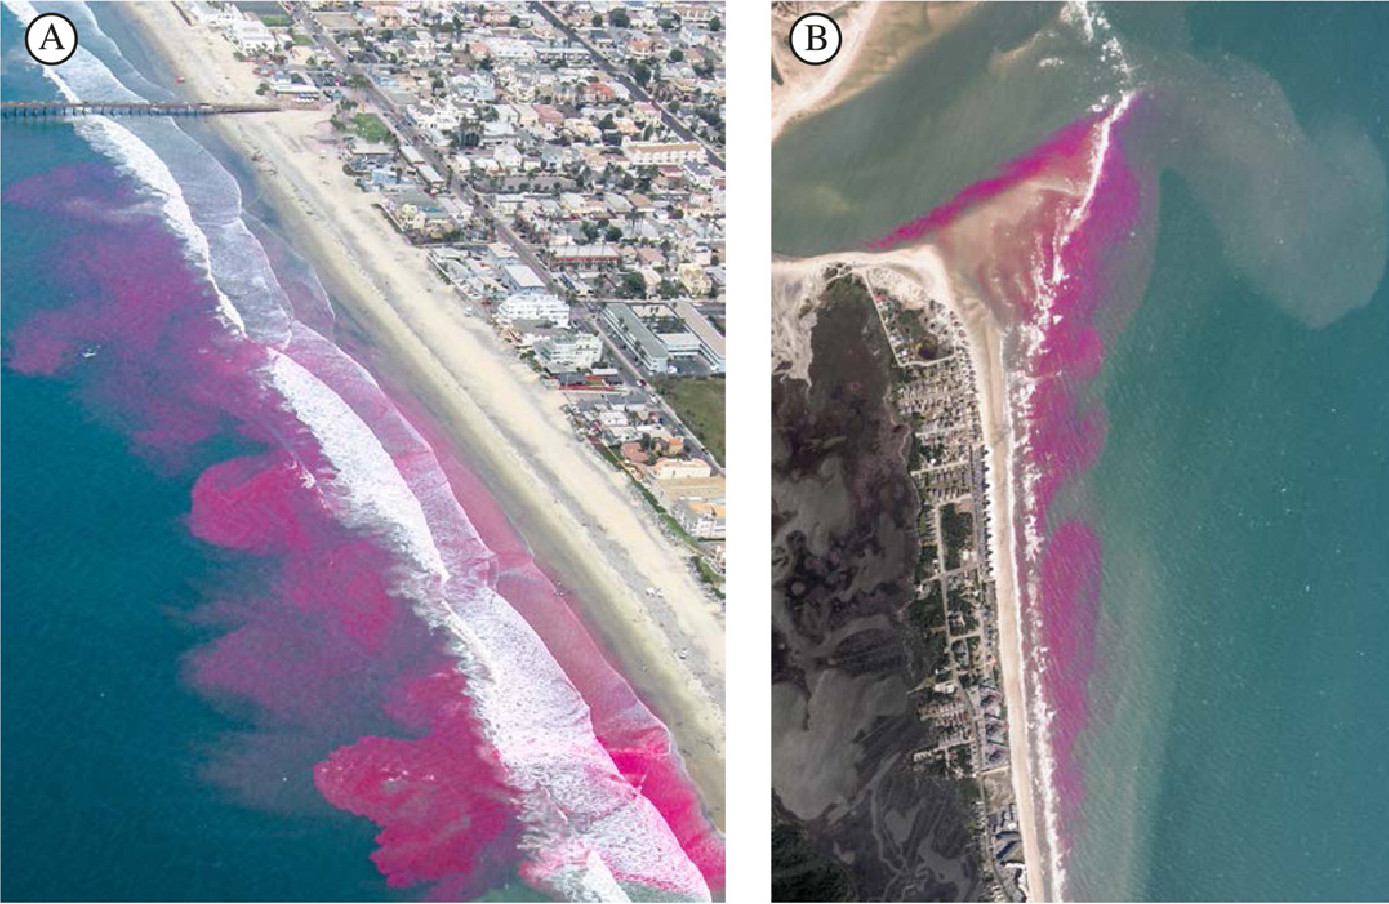
\includegraphics[width=0.9\textwidth]{FIGURES/surf_zone_pink.jpg}}
%\vspace{3.64in}
  \caption{Longshore and cross-shore transport in the surf zone. (A) shows a release in the surfzone at Imperial Beach, south of San Diego, California,
and (B) shows a release within an ebb tidal flow at New River Inlet, North Carolina. Figure from \cite{Clark&al.2014}, copyright American Meteorological Society.}
    {}
\label{fig:surf_pink}
\end{figure}
%%%%%%%%%%%%% end of figure



%\section{Séparation des qdm vagues et circulation}
%Les deux termes en $S^J$ dans (\ref{Garrett}) représentent la pression moyenne induite par les vagues, qui agit logiquement sur la circulation moyenne, et une force supplémentaire $\rho_w  S^J \partial D / \partial x_\alpha$ qui compense la force $-\rho_w   S^J \partial D / \partial x_\alpha$ qui agit sur la PQDM dans (\ref{wavemom}).  Il apparaît donc que ce deuxième terme est une interaction entre la circulation moyenne et l'état de mer, il n'y a donc pas d'interaction avec le fond. Ainsi, en absence de frottement sur le fond et sans réflexion des vagues, la force moyenne exercée par le fond sur la colonne d'eau n'est que la pression hydrostatique. Il n'y a pas de force moyenne sur l'écoulement susceptible de modifier la quantité de mouvement des vagues ou de l'écoulement moyen et la réfraction et le levage ne sont pas la conséquence d'une force exercée par le fond, mais seulement le résultat d'une modification du guide d'onde, sans échange d'énergie ou de quantité de mouvement avec l'extérieur (Longuet-Higgins 1967,1977\nocite{Longuet-Higgins1967,Longuet-Higgins1977}, Ardhuin 2006\nocite{Ardhuin2006b}).

%%%%%%%%%%%%% figure
%\begin{figure}
%\centerline{\includegraphics[width=0.8\textwidth]{FIGURES/wave_over_step.pdf}}
%  \caption{Equilibre des forces pour des vagues au-dessus d'une marche
%  lissée.}{En absence de réflexion et de dissipation des vagues, la  force correspondant à la divergence du flux de quantité de mouvement induit par les vagues se combine   avec la pression moyenne. Cette combinaison est généralement équilibrée par un gradient de pression hydrostatique associé   au gradient de la surface libre. L'accélération de la circulation moyenne   (petites flèches en pointillés) n'apporte, en général, qu'une faible  correction à cet équilibre. En absence de réflexion, il n'y a pas de force exercée par le fond, outre la pression hydrostatique.} \label{fig_wave_over_step}
%\end{figure}
%%%%%%%%%%%%% end of figure

%On peut alors reconsidérer le problème de vagues unidirectionnelles se propageant au-dessus d'une marche d'escalier lissée avec un changement de profondeur de $h_1$ à $h_2$  (Whitham 1962, section 2\nocite{Whitham1962}). Nous sommes d'accord avec Whitham sur la conservation du flux de masse $E_1/C_1 +\rho_w (h_1 + \overline{\zeta}_1)U_1 = E_2/C_2 +\rho_w (h_2 + \overline{\zeta}_2)U_2$, mais par contre, pour la quantité de mouvement notre conclusion est différente de la sienne. La différence de flux de PQDM $C_{g2}/C_2 E_2 - C_{g1}/C_1 E_1$ ne correspond pas à la force exercée sur la marche, comme suggéré par Whitham, mais à une force exercée sur l'écoulement moyen, à laquelle s'ajoute le gradient de la pression induite par les vagues $S^J$ pour donner les tensions de radiation classiques. Dans le cas d'une dissipation négligeable, l'ensemble des deux termes est compensé par une variation de la surface libre: la décôte (figure \ref{fig_wave_over_step}). Cette conclusion est vérifiée expérimentalement par les mesures de la dépression du niveau moyen faites par Saville (1961\nocite{Saville1961}, voir aussi l'analyse faite par Longuet-Higgins and Stewart 1963\nocite{Longuet-Higgins&Stewart1963}, et Phillips 1977) et Bowen et coll. (1968\nocite{Bowen&al.1968}).

%En outre il doit aussi y a avoir une divergence de la circulation moyenne pour compenser la divergence de la dérive de Stokes. Toutefois, la divergence correspondante de quantité de mouvement moyen (flèches courtes en pointillés sur la figure \ref{fig_wave_over_step}) est généralement beaucoup plus faible  que les tensions de radiation à cause du rapport des flux de quantité de mouvement et de masse des vagues, qui est égal à la vitesse de groupe $C_g$, qui est en générale plus grande que le rapport correspondant pour la circulation moyenne, égal au courant en moyenne verticale. Dans des cas ou la réflexion des vagues est importante, la force de diffusion  ${\mathbf T}^{\mathrm{bscat}}$ doit aussi être prise en compte car elle est exercée par le fond, et annule la partie correspondante de la divergence du flux de quantité de mouvement.

%On doit donc clairement séparer trois forces horizontales induites par les vagues,
%\begin{itemize} 
%  \item la force de pression induite par les vagues, qui est typiquement équilibrée par la décôte dans les cas conservatifs.  Après intégration sur la vertical elle est égale à  $-\rho_w  \partial S^J/\partial x_\alpha$.
%  \item la force de vortex qui est due au cisaillement de courant et à l'advection croisée  de quantité de mouvement des vagues par le courant et du courant par les vagues
%  \item la force exercée sur la circulation moyenne correspondant à la divergence de la pseudo-quantité de mouvement (PQDM), corrigée des effets de réflexion des vagues par la topographie, et  de la perte de PQDM par frottement sur le fond.
%\end{itemize}
%En effet, la fraction de la PQDM perdue par frottement sur le fond n'est que temporairement communiquée à la circulation, en contribuant au courant de ruissellement  (Russel and Osorio 1958\nocite{Russel&Osorio1958}), avant de finir dans le fond via un cisaillement moyen (Longuet-Higgins 2005).

%%%%%%%%%%%%% figure
%\begin{figure}
%\centerline{\includegraphics[width=0.8\textwidth]{FIGURES/NTUA2_meanflow.pdf}}
%  \caption{Ecoulements Eulériens et Lagrangiens moyens pour des vagues au-dessus d'une marche  lissée.}{(a) Perturbation de pression $(p-\overline{p})/(\rho_w g)$ à $t=0$  telle que calculée avec le modèle NTUA-nl2 (Belibassakis and Athanassoulis 2002), qui résoud l'équation de Laplace à l'ordre 2 en pente des   vagues, pour des vagues d'amplitude $a=0.12$~m.  (b) Courant Eulérien moyen $-\widehat{u}$, et (c) composante horizontale de la pseudo-quantité de mouvement $P_1$, qui est ici égale à la dérive de Stokes. Les flèches indiquent le sens de l'écoulement.} \label{fig_NTUA2}
%\end{figure}
%%%%%%%%%%%%% end of figure

